\documentclass[tikz,border=7pt]{standalone}
\usepackage{libertinus}
\usepackage{amsmath}
\usetikzlibrary{
  arrows.meta,
  backgrounds,
  calc,
  decorations.markings,
  fit,
  positioning
}

\definecolor{accent}{RGB}{38,103,115}
\definecolor{softgray}{RGB}{244,245,246}
\definecolor{midgray}{RGB}{123,128,132}

\tikzset{
  >={Latex[length=2.2mm,width=1.5mm]},
  flow/.style={-Latex,semithick,draw=black!72},
  accent flow/.style={-Latex,semithick,draw=accent},
  box/.style={
    draw=black!68,
    fill=softgray,
    rounded corners=1.2pt,
    align=center,
    inner xsep=5pt,
    inner ysep=4pt
  },
  accent box/.style={
    draw=accent,
    fill=accent!8,
    rounded corners=1.2pt,
    align=center,
    inner xsep=5pt,
    inner ysep=4pt
  },
  point/.style={circle,draw=black!75,fill=white,inner sep=1.7pt},
  accent point/.style={circle,draw=accent,fill=accent!10,inner sep=1.7pt},
  tinylabel/.style={font=\scriptsize,align=center},
  smalllabel/.style={font=\small,align=center},
  panel/.style={draw=black!28,rounded corners=2pt,inner sep=6pt}
}


\begin{document}
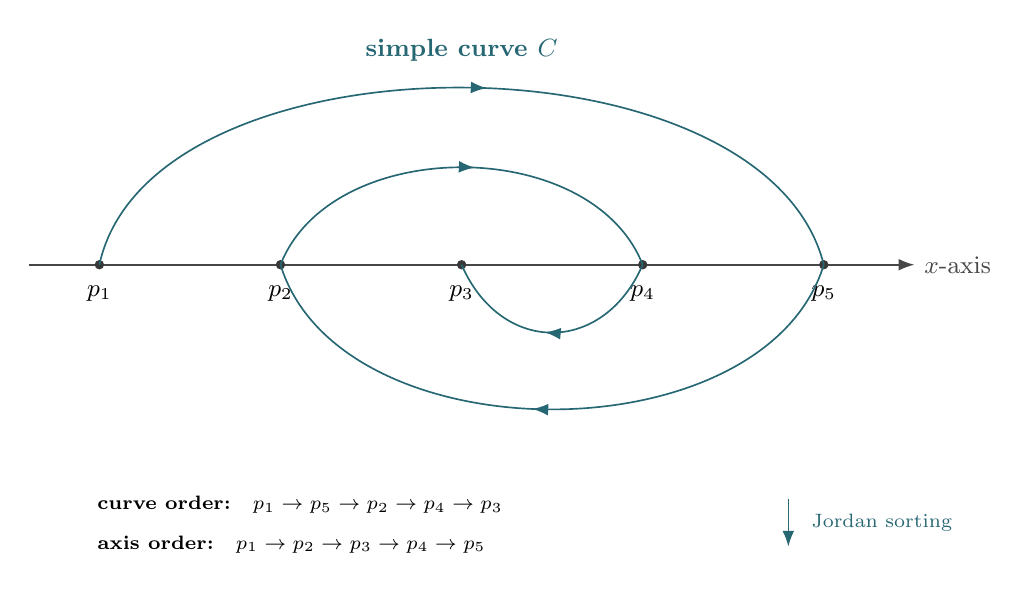
\begin{tikzpicture}[x=1cm,y=1cm,font=\small]
  \coordinate (p1) at (0.8,0);
  \coordinate (p2) at (3.1,0);
  \coordinate (p3) at (5.4,0);
  \coordinate (p4) at (7.7,0);
  \coordinate (p5) at (10.0,0);

  \draw[black!72,semithick,-Latex] (-0.1,0) -- (11.15,0)
    node[right,font=\small] {$x$-axis};

  \foreach \p/\name in {p1/$p_1$,p2/$p_2$,p3/$p_3$,p4/$p_4$,p5/$p_5$} {
    \fill[black!78] (\p) circle (1.7pt);
    \node[below=4pt] at (\p) {\name};
  }

  \tikzset{curve/.style={
    semithick,
    draw=accent,
    postaction={decorate},
    decoration={markings,mark=at position .53 with {\arrow{Latex}}}
  }}
  \draw[curve] (p1) .. controls (1.45,3.0) and (9.25,3.0) .. (p5);
  \draw[curve] (p5) .. controls (9.25,-2.45) and (3.85,-2.45) .. (p2);
  \draw[curve] (p2) .. controls (3.75,1.65) and (7.05,1.65) .. (p4);
  \draw[curve] (p4) .. controls (7.2,-1.15) and (5.9,-1.15) .. (p3);

  \node[accent,text=accent,font=\small\bfseries] at (5.4,2.72) {simple curve $C$};
  \node[font=\scriptsize,align=left,anchor=west] at (0.65,-3.05) {
    \textbf{curve order:}\quad
    $p_1 \rightarrow p_5 \rightarrow p_2 \rightarrow p_4 \rightarrow p_3$
  };
  \node[font=\scriptsize,align=left,anchor=west] at (0.65,-3.55) {
    \textbf{axis order:}\quad
    $p_1 \rightarrow p_2 \rightarrow p_3 \rightarrow p_4 \rightarrow p_5$
  };

  \draw[accent flow] (9.55,-2.98) -- (9.55,-3.58);
  \node[font=\scriptsize,text=accent,anchor=west] at (9.72,-3.28)
    {Jordan sorting};
\end{tikzpicture}
\end{document}
